\documentclass{article}
\usepackage{amsmath}
\usepackage{amssymb}
\usepackage{ctex}
\usepackage[margin=2cm]{geometry} % 设置较窄的边距使文档宽一些
\usepackage{multirow} % 支持表格中的多行单元格
\usepackage{graphicx} % 用于插入图片
\usepackage{subcaption} % 支持子标题
\usepackage{float} % 支持 [H] 浮动体选项
\title{\heiti\zihao{2}实验四 \quad 三相电路功率的测量}
\author{\songti  author  Student ID  \\
课程号  XXXXXX.01 }
\date{2025.5.26}
\begin{document}
    \maketitle
\begin{abstract}
    \noindent{\textbf{摘要:} 本实验主要研究三相电路功率的测量方法,包括一瓦特表法和二瓦特表法。通过实验,掌握了如何使用功率表测量三相电路的有功功率和无功功率,并进一步熟悉功率表的接线和使用方法。实验结果验证了理论知识,并加深了对三相电路功率测量的理解。}
    
    \noindent{\textbf{关键词:} 三相电路;功率测量;一瓦特表法;二瓦特表法;有功功率;无功功率}
\end{abstract}
\section{实验目的}
\begin{enumerate}
    \item 掌握用一瓦特表法、二瓦特表法测量三相电路有功功率与无功功率的方法
    \item 进一步熟练掌握功率表的接线和使用方法
\end{enumerate}

\section{实验原理}
1.对于三相四线制供电的三相星形联接的负载(即 $\mathrm{Y}_{\mathrm{o}}$ 接法),可用一只功率表测量各相的有功功率 $\mathrm{P}_{\mathrm{A}} 、 \mathrm{P}_{\mathrm{B}} 、 \mathrm{P}_{\mathrm{C}}$ ,则三相负载的总有功功率 $\Sigma \mathrm{P}=\mathrm{P}_{\mathrm{A}}+\mathrm{P}_{\mathrm{B}}+\mathrm{P}_{\mathrm{C}}$ 。这就是一瓦特表法,如图 4-1 所示。若三相负载是对称的,则只需测量一相的功率,再乘以 3 即得三相总的有功功率。

2.三相三线制供电系统中,不论三相负载是否对称,也不论负载是 Y 接还是 $\triangle$ 接,都可用二瓦特表法测量三相负载的总有功功率。若负载为感性或容性,且当相位差 $\phi>60^{\circ}$ 时,线路中的一只功率表指针将反偏(数字式功率表将出现负读数),这时应将功率表电流线圈的两个端子调换(不能调换电压线圈端子),其读数应记为负值。而三相总功率 $\sum$ $\mathrm{P}=\mathrm{P}_1+\mathrm{P}_2$( $\mathrm{P}_1 、 \mathrm{P}_2$ 本身不含任何意义)。
\begin{figure}[H]
    \centering
    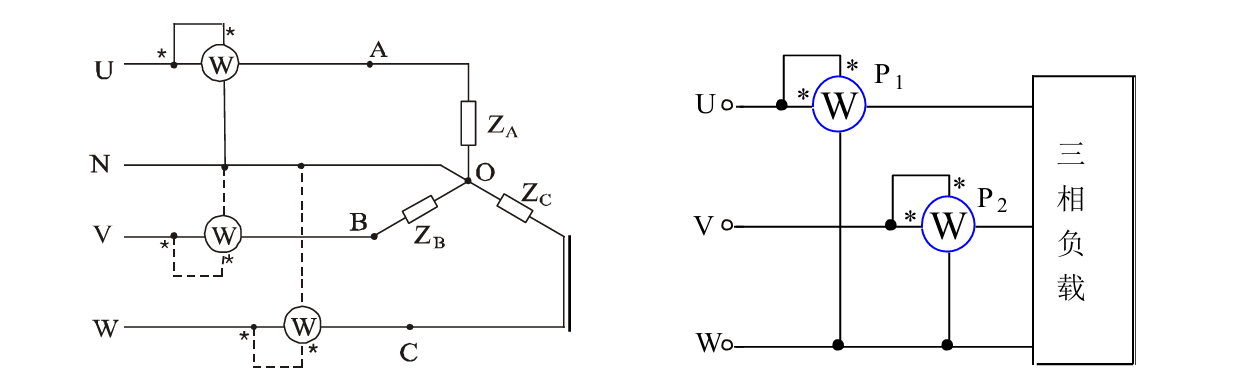
\includegraphics[width=0.8\textwidth]{img1.png}
    \caption{二瓦特表法测量三相负载的总有功功率}
\end{figure}



除了图 2 的 $\mathrm{I}_A 、 \mathrm{U}_{A C}$ 与 $\mathrm{I}_B 、 \mathrm{U}_{B C}$ 接法外,还有 $\mathrm{I}_B 、 \mathrm{U}_{A B}$ 与 $\mathrm{I}_C 、 \mathrm{U}_{A C}$ 以及 $\mathrm{I}_A 、 \mathrm{U}_{A B}$ 与 $\mathrm{I}_C 、 \mathrm{U}_{B C}$两种接法。

3.对于三相三线制供电的三相对称负载,可用一瓦特表法测得三相负载的总无功功率 Q,测试原理线路如图 2 所示。

\begin{figure}[H]
    \centering
    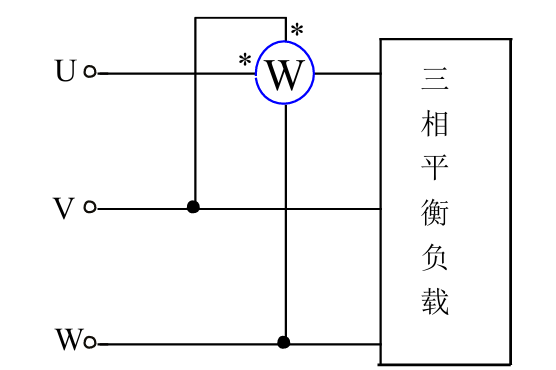
\includegraphics[width=0.5\textwidth]{img2.png}
    \caption{一瓦特表法测总无功功率}
\end{figure}


图示功率表读数的 $\sqrt{3}$ 倍,即为对称三相电路总的无功功率。除了此图给出的一种连接法( $\mathrm{I}_{\mathrm{U}} 、 \mathrm{U}_{\mathrm{VW}}$ )外,还有另外两种连接法,即接成( $\mathrm{I}_{\mathrm{V}} 、 \mathrm{U}_{\mathrm{UW}}$ )或( $\mathrm{I}_{\mathrm{W}} 、 \mathrm{U}_{\mathrm{UV}}$ )。

\section{实验器材}
\label{sec:equipment}
    \begin{enumerate}
        \item 交流电压表  0~500V 
        \item 交流电流表 0~5A 
        \item 单相功率表 
        \item 万用表
        \item 三相自耦调压器 
        \item 三相灯组负载 220V,25W 白炽灯 
        \item 三相电容负载 $1 \mu \mathrm{~F}, \quad 2.2 \mu \mathrm{~F}, \quad 4.7 \mu \mathrm{~F} / 500 \mathrm{~V}$
    \end{enumerate} 

\section{实验内容}
\subsection{ 用一瓦特表法测定三相对称 Y0 接以及不对称 Y0 接负载的总功率$\Sigma$P。}

实验按图 3 线路
接线。线路中的电流表和电压表用以监视该相的电流和电压,不要超过功率表电压和电流的量程。 
经指导教师检查后,接通三相电源,调节调压器输出,使输出线电压为 220V,按表 4-1 的要
求进行测量及计算。

\begin{figure}[H]
    \centering
    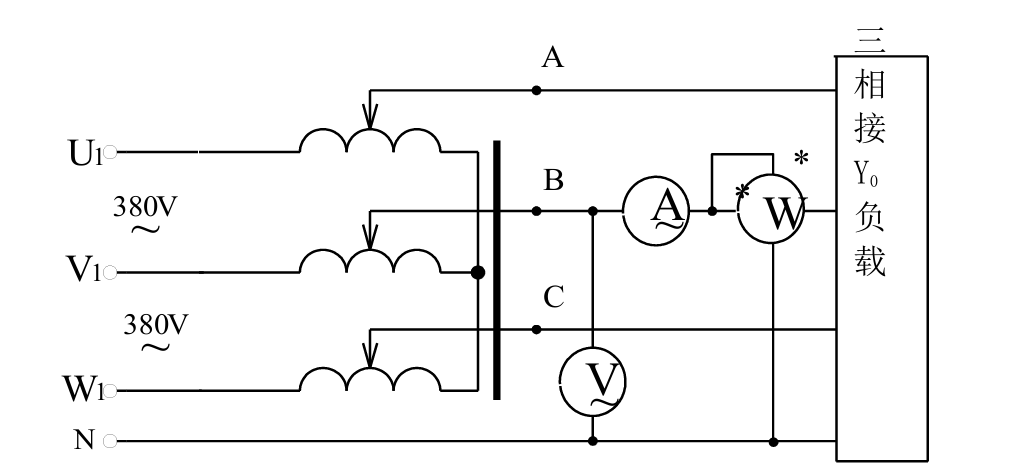
\includegraphics[width=0.8\textwidth]{img3.png}
    \caption{一瓦特表法测定三相对称 Y0 接以及不对称 Y0 接负载的总功率$\Sigma$P}
\end{figure}



\begin{tabular}{|l|l|l|l|l|l|l|l|}
\hline \multirow{2}{*}{负载情况} & \multicolumn{3}{|c|}{开灯盏数} & \multicolumn{3}{|c|}{测量数据} & 计算值 \\
\hline & A 相 & B 相 & C 相 & $\mathrm{P}_{\mathrm{A}}$ (W) & $\mathrm{P}_{\mathrm{B}}$ (W) & $\mathrm{P}_{\mathrm{C}}$ (W) & $\Sigma \mathrm{P}$ (W) \\
\hline $\mathrm{Y}_0$ 接对称负载 & 3 & 3 & 3 & 31.9& 34.7& 32.9&99.5 \\
\hline $\mathrm{Y}_0$ 接不对称负载 & 1 & 2 & 3 &10.9 &23.5 &32.7 & 67.1\\
\hline
\end{tabular}
\subsection{用二瓦特表法测定三相负载的总功率 }

(1)按图 4 接线,将三相灯组负载接成 Y 形接法。

\begin{figure}[H]
    \centering
    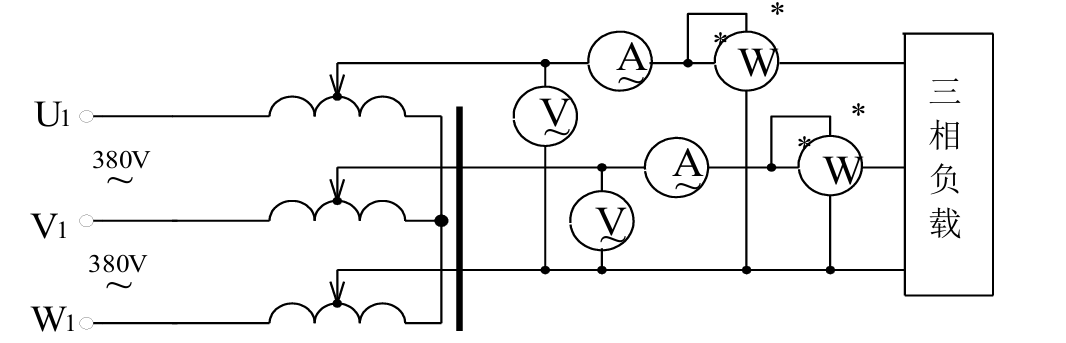
\includegraphics[width=0.8\textwidth]{img4.png}
    \caption{二瓦特表法测定三相负载的总功率}
\end{figure}

经指导教师检查后,接通三相电源,调节调压器的输出线电压为 220V,按表 2 的内容进
行测量。

(2)将三相灯组负载改成 $\triangle$ 形接法,重复(1)的测量步骤,数据记入表 2 中。

\begin{tabular}{|l|l|l|l|l|l|l|}
\hline \multirow{2}{*}{负载情况} & \multicolumn{3}{|c|}{开灯盏数} & \multicolumn{2}{|c|}{测量数据} & 计算值 \\
\hline & A 相 & B 相 & C 相 & $\mathrm{P}_1$ (W) & $\mathrm{P}_2$ (W) & $\Sigma \mathrm{P}$ (W) \\
\hline Y 接平衡负载 & 3 & 3 & 3 &48.1 &51.3 &99.4 \\
\hline Y 接不平衡负载 & 1 & 2 & 3 & 20.3& 41.7& 62.0\\
\hline $\triangle$ 接平衡负载 & 3 & 3 & 3 &110.9 &111.1 &222.0 \\
\hline $\triangle$ 接不平衡负载 & 1 & 2 & 3 & 87.1&98.9 &186 \\
\hline
\end{tabular}

\section{预习思考题 }


\subsection{测量功率时为什么在线路中通常都接有电流表和电压表?  }

因为功率是电压与电流的乘积,即 P=UI。
测量功率时电流表串联在电路中是为了测出流过电路的电流 I;把电压表并联在电路中是为了测出加在负载两端的电压 U;再把测出的数值代入上式即可算出功率。


\section{总结感悟 }
本次实验通过一瓦特表法和二瓦特表法测量三相电路的功率,深入理解了三相电路功率测量的原理和方法。通过实际操作,掌握了功率表的接线和使用技巧,增强了对三相电路的理解。实验结果与理论预期一致,验证了功率测量方法的正确性。

\section{参考文献}
\begin{enumerate}
    \item 电子电路实验指导书
    \item 电子电路基础
    \item 电路原理
    \item 电路分析
\end{enumerate} 



\end{document}